\documentclass[journal]{vgtc}                     % final (journal style)
%\documentclass[journal,hideappendix]{vgtc}        % final (journal style) without appendices
% \documentclass[review,journal]{vgtc}              % review (journal style)
% \documentclass[review,journal,hideappendix]{vgtc} % review (journal style)
%\documentclass[widereview]{vgtc}                  % wide-spaced review
%\documentclass[preprint,journal]{vgtc}            % preprint (journal style)


%% Uncomment one of the lines above depending on where your paper is
%% in the conference process. ``review'' and ``widereview'' are for review
%% submission, ``preprint'' is for pre-publication in an open access repository,
%% and the final version doesn't use a specific qualifier.

%% If you are submitting a paper to a conference for review with a double
%% blind reviewing process, please use one of the ``review'' options and replace the value ``0'' below with your
%% OnlineID. Otherwise, you may safely leave it at ``0''.
\onlineid{5446}

%% In preprint mode you may define your own headline. If not, the default IEEE copyright message will appear in preprint mode.
%\preprinttext{To appear in IEEE Transactions on Visualization and Computer Graphics.}

%% In preprint mode, this adds a link to the version of the paper on IEEEXplore
%% Uncomment this line when you produce a preprint version of the article 
%% after the article receives a DOI for the paper from IEEE
%\ieeedoi{xx.xxxx/TVCG.201x.xxxxxxx}

%% declare the category of your paper, only shown in review mode
\vgtccategory{Research}

%% Paper title.
\title{TPS-Vis: Interactive Visual Exploration of PD-L1 Expression in Lung Cancer Pathology Images}

%% Author ORCID IDs should be specified using \authororcid like below inside
%% of the \author command. ORCID IDs can be registered at https://orcid.org/.
%% Include only the 16-digit dashed ID.
\author{%
  Yuning Hu$^{\dagger}$, Liting Fang$^{\dagger}$, Ruiqi Yang, Jingyu Li, Zhenyang Wang, Wei Zhang,  
  Zunlei Feng, Chaoqing Xu* 
}


\authorfooter{
  %% insert punctuation at end of each item
  \item
  	Y. Hu, W. Zhang, C. Xu, L. Fang, and J. Li are with Hangzhou City University.
  	E-mail: \{huyuning, zw_yixian, xucq\}@hzcu.edu.cn, flting.amanda@gmail.com,  \\ 32401203@stu.hzcu.edu.cn

  \item R. Yang and Z. Feng are with Zhejiang University.
  	E-mail: rickyyang0113@gmail.com, zunleifeng@zju.edu.cn. 

  \item Z. Wang is with N-Dimension Tech Co.
  	E-mail: wangzhenyang@swpatho.com. 
    
  \item
  $^{\dagger}$ Yuning Hu and Liting Fang contributed equally to this work.
  \item
  * Corresponding authors: Chaoqing Xu.
}

%% Abstract section.
\abstract{%
  % 在肺癌的临床免疫治疗中，医生通常基于免疫组织化学（IHC）切片评估肿瘤组织中的 PD-L1 表达状态，并将肿瘤比例评分（TPS）作为辅助治疗方案选择的重要参考。然而，在实际临床流程中，TPS 评估高度依赖病理医生经验，医生需要在全切片图像中反复缩放，定位肿瘤区域并核查细胞膜染色状态，评估结果容易受到肿瘤与非肿瘤区域混杂、坏死组织和弱阳性表达等因素影响。为此，本文提出一个面向肺癌 PD-L1 的交互式可视分析系统。系统支持多层级 PD-L1 表达状态识别，通过多尺度联动可视化呈现全局与局部的阳性、阴性分布，并自动计算 TPS 指标，帮助医生更高效地完成肿瘤区域核查、细胞级证据追溯和量化评估，从而实现更加智能、快捷、稳定和可解释的 PD-L1 辅助判读。
In clinical immunotherapy for lung cancer, pathologists commonly assess PD-L1 expression status from IHC slides and use the TPS as an important reference for treatment selection. However, in routine clinical workflows, TPS assessment remains highly dependent on pathologists’ experience. Experts need to repeatedly zoom in and out on whole-slide images, locate tumor regions, and inspect membranous staining patterns at the cellular level. This process is easily affected by mixed tumor and non-tumor regions, necrotic tissues, weak positive expression, and other complex pathological factors. To address these challenges, this paper presents an interactive visual analytics system for PD-L1 assessment in lung cancer pathology. The system supports multi-level identification of PD-L1 expression states, presents global and local distributions of positive and negative regions through coordinated multi-scale visualization, and automatically computes TPS. The system helps pathologists perform tumor-region verification, cell-level evidence review, and quantitative TPS assessment more efficiently, thereby improving the consistency, interpretability, and usability of PD-L1-assisted pathological interpretation.}

%% Keywords that describe your work. Will show as 'Index Terms' in journal
%% please capitalize first letter and insert punctuation after last keyword
\keywords{PD-L1 Assessment, Tumor Proportion Score, Digital Pathology, Visual Analytics, Multi-scale Visualization.}

%% A teaser figure can be included as follows
\teaser{
  \centering
      
\includegraphics[width=\linewidth]{figs/Teaser.png}
  \caption{%
  The interface of our interactive PD-L1 visual analytics system for lung cancer pathology images comprises (A) a specimen explorer, (B) a patch gallery, (C) a multi-scale focus view of the whole-slide image with region of interest (ROI) selection and overlayed TPS heatmap, (D) a cohort-level quantitative dashboard including (D-1) a fine-grained TPS histogram and (D-2) selection-linked summary statistics, (E) a cell-level evidence inspection panel featuring (E-1) cell type maps, (E-2) cell probability maps, and (E-3) detailed patch-level statistics with weighted TPS and cell counts, and (F) the Pathology Insight Agent.
  }
  \label{fig:teaser}
}

%% Uncomment below to disable the manuscript note
%\renewcommand{\manuscriptnotetxt}{}

%% Copyright space is enabled by default as required by guidelines.
%% It is disabled by the 'review' option or via the following command:
%\nocopyrightspace


%%%%%%%%%%%%%%%%%%%%%%%%%%%%%%%%%%%%%%%%%%%%%%%%%%%%%%%%%%%%%%%%
%%%%%%%%%%%%%%%%%%%%%% LOAD PACKAGES %%%%%%%%%%%%%%%%%%%%%%%%%%%
%%%%%%%%%%%%%%%%%%%%%%%%%%%%%%%%%%%%%%%%%%%%%%%%%%%%%%%%%%%%%%%%

%% Tell graphicx where to find files for figures when calling \includegraphics.
%% Note that due to the \DeclareGraphicsExtensions{} call it is no longer necessary
%% to provide the the path and extension of a graphics file:
%% 
\includegraphics{diamondrule} is completely sufficient.
\graphicspath{{figs/}{figures/}{pictures/}{images/}{./}} % where to search for the images

%% Only used in the template examples. You can remove these lines.
\usepackage{tabu}                      % only used for the table example
\usepackage{booktabs}                  % only used for the table example
\usepackage{lipsum}                    % used to generate placeholder text
\usepackage{mwe}                       % used to generate placeholder figures
\usepackage{ccicons}                   % package to be able to use icons from creative commons
\usepackage{amsmath}
\usepackage{amssymb}
%% We encourage the use of mathptmx for consistent usage of times font
%% throughout the proceedings. However, if you encounter conflicts
%% with other math-related packages, you may want to disable it.
\usepackage{mathptmx}                  % use matching math font
\usepackage{dblfloatfix} % 导言区
\usepackage{xcolor}

\begin{document}

%%%%%%%%%%%%%%%%%%%%%%%%%%%%%%%%%%%%%%%%%%%%%%%%%%%%%%%%%%%%%%%%
%%%%%%%%%%%%%%%%%%%%%% START OF THE PAPER %%%%%%%%%%%%%%%%%%%%%%
%%%%%%%%%%%%%%%%%%%%%%%%%%%%%%%%%%%%%%%%%%%%%%%%%%%%%%%%%%%%%%%%

%% The ``\maketitle'' command must be the first command after the
%% ``\begin{document}'' command. It prepares and prints the title block.
%% the only exception to this rule is the \firstsection command

\maketitle

\firstsection{Introduction}
%     肺癌是全球范围内发病率和死亡率均较高的恶性肿瘤之一，免疫治疗已成为其临床治疗中的重要手段。作为免疫治疗决策的重要依据，程序性死亡配体 1（programmed death-ligand 1, PD-L1）的表达水平通常通过免疫组织化学（immunohistochemistry, IHC）切片进行评估。其中，肿瘤比例评分（tumor proportion score, TPS）是肺癌 PD-L1 判读中常用的量化指标，其核心在于估计具有膜性 PD-L1 染色的肿瘤细胞在全部存活肿瘤细胞中的比例\cite{herbst2014predictive}。准确的 TPS 评估能够为患者分层和治疗方案选择提供重要参考。因此，如何在高分辨率病理切片中高效、稳定地识别 PD-L1 表达状态，并辅助医生完成可信的 TPS 判读，是数字病理和临床免疫治疗中的重要问题。
%         在实际临床流程中，TPS 判读仍高度依赖病理医生的经验。医生通常需要在超大尺寸的全切片图像中缩放和平移，首先定位肿瘤区域，再进一步观察局部区域中肿瘤细胞的膜染色情况，并根据经验对 TPS 进行肉眼估计。与直接计算阳性细胞比例不同，TPS 判读的关键并不仅在于识别 PD-L1 阳性细胞，更在于准确确定有效肿瘤区域和存活肿瘤细胞。在不同图像区域中，可能同时存在坏死组织、炎性细胞浸润、肿瘤与非肿瘤成分混杂等复杂情况；弱阳性表达、细胞密集分布、染色强度波动以及不同肺癌组织学亚型差异，也会进一步增加判读难度。医生通过肉眼进行粗略估计会导致出现判读差异。
%         近年来，人工智能方法在数字病理图像分析中取得了快速发展，并在组织分割、细胞检测、病理分类和预后预测等任务中展现出较强能力\cite{zhang2024efficient,chen2024towards}。对于 PD-L1 IHC 图像，已有方法能够进行 patch 级表达状态分类、肿瘤区域识别或细胞级阳性/阴性判别\cite{mclaughlin2016quantitative,liu2021automated}，也有若干 TPS 计算工具被用于数字病理分析\cite{huang2022new}。然而，现有方法多侧重单一层级的自动识别或最终评分输出，无法进行多层级TPS可视化追溯和精细化判读。病理专家不仅需要知道 TPS 得分，还需要理解该得分来源于哪些肿瘤区域、哪些局部细胞分布模式。具体而言，PD-L1 辅助判读仍面临以下挑战。首先，病理切片标注成本高昂，细胞级标注和显式分割容易受到图像质量、细胞重叠和染色差异的影响，如何在全切片级图像中实现高效、稳定的多层级状态识别和 TPS 计算仍然具有挑战。其次，PD-L1 IHC 全切片图像通常具有超高分辨率和显著的多尺度特征，如何在全局分布、区域结构和细胞细节之间切换与联动分析也是一个重要问题。第三，单一 TPS 数值难以充分呈现评分背后的空间依据和细胞证据，如何帮助医生追溯评分来源并核查关键区域，是提升辅助判读可信度的关键。因此，临床研究亟需一种具备快速计算和全局追溯的交互式 PD-L1 表达辅助判读系统。
%         可视分析是一种结合数据挖掘、人机交互和可视化技术的分析方法。通过将人工智能模型、量化统计分析和交互式可视化相结合，其能够把复杂的全切片图像和算法结果转化为医生可理解、可核查和可操作的视觉证据。基于此，本文提出一个面向肺癌 PD-L1 表达评估的交互式可视分析系统。系统支持从全片到细胞级的 PD-L1 表达状态识别，实现TPS 的一致性计算；通过多尺度联动视图，系统呈现全切片、patch 和细胞层面的 PD-L1 表达分布，实现可信评估。医生还可以手动选择感兴趣区域，系统自动生成 TPS 相关统计结果和可视化图表，实现灵活筛选和按需细查。最后提供Agent交互式问答，提高判读效率，实现智能、快捷、稳定和可解释的 PD-L1 辅助评估。本文的主要贡献如下：
% 1. 提出一套多层级 PD-L1 表达联合建模方法，能够同时支持 patch-level 表达分类和细胞级阳性/阴性判别，实现高效快速的多尺度TPS计算和细胞状态识别。
% 2. 提出一个面向肺癌 PD-L1 表达评估的交互式可视分析系统，支持从全片到细胞级的多层级判读、感兴趣区域选择、量化分析和智能评估，实现复杂切片的高效交互探索。
% 3. 基于真实肺癌 PD-L1 IHC 数据开展案例分析，结果表明该系统能够直观辅助专家进行切片浏览、筛查和判读分析，提升评估过程的一致性与效率。

Lung cancer is one of the most prevalent and deadly malignancies worldwide, and immunotherapy has become an important component of its clinical treatment. As a critical reference for immunotherapy decision-making, the expression level of programmed death-ligand 1 (PD-L1) is commonly assessed using immunohistochemistry (IHC) slides. Among the quantitative criteria used for PD-L1 interpretation in lung cancer, the tumor proportion score (TPS) is widely adopted. It estimates the proportion of viable tumor cells showing membranous PD-L1 staining among all viable tumor cells\cite{herbst2014predictive}. Accurate TPS assessment provides important evidence for patient stratification and treatment selection. Therefore, efficiently and robustly identifying PD-L1 expression patterns in high-resolution pathology slides and assisting physicians in reliable TPS interpretation remain important challenges in digital pathology and clinical immunotherapy.

In clinical practice, TPS interpretation still heavily relies on the experience of pathologists. Physicians usually need to zoom and pan across ultra-large whole-slide images, first locating tumor regions and then examining membranous staining patterns of tumor cells in local areas, before visually estimating the TPS based on their expertise. Unlike a straightforward calculation of the proportion of positive cells, TPS interpretation depends not only on the identification of PD-L1-positive cells, but also on the accurate determination of valid tumor regions and viable tumor cells. Different regions of a slide may contain necrotic tissue, inflammatory cell infiltration, and mixtures of tumor and non-tumor components. In addition, weak positive expression, densely distributed cells, variations in staining intensity, and differences among lung cancer histological subtypes further increase the difficulty of interpretation. Such visual and semi-quantitative estimation may lead to inter-observer variability.

In recent years, artificial intelligence methods have advanced rapidly in digital pathology image analysis, demonstrating strong capabilities in tissue segmentation, cell detection, pathological classification, and prognosis prediction\cite{zhang2024efficient,chen2024towards}. For PD-L1 IHC images, existing methods can perform patch-level expression classification, tumor region recognition, or cell-level positive/negative discrimination\cite{mclaughlin2016quantitative,liu2021automated}, and several TPS calculation tools have also been used in digital pathology analysis\cite{huang2022new}. However, most existing methods focus on automatic recognition at a single level or on producing a final score, and they provide limited support for multi-level visual tracing and fine-grained TPS interpretation. Pathologists need not only the TPS value, but also an understanding of which tumor regions and local cellular distribution patterns contribute to the score.

Specifically, PD-L1-assisted interpretation still faces several challenges. First, annotation of pathology slides is costly, and cell-level labeling and explicit segmentation are easily affected by image quality, cell overlap, and staining variations. It remains challenging to achieve efficient and robust multi-level state recognition and TPS calculation on whole-slide images. Second, PD-L1 IHC whole-slide images are typically characterized by ultra-high resolution and prominent multi-scale structures, making it important to support coordinated analysis across global distributions, regional structures, and cellular details. Third, a single TPS value cannot sufficiently reveal the spatial evidence and cellular basis underlying the score. Helping physicians trace the source of the score and verify key regions is therefore essential for improving the reliability of assisted interpretation. Accordingly, clinical research urgently requires an interactive PD-L1 expression assessment approach that supports rapid computation and global evidence tracing.

Visual analytics, which integrates data mining, human-computer interaction, and visualization techniques, provides an effective solution to this problem. By combining artificial intelligence models, quantitative statistical analysis, and interactive visualization, visual analytics can transform complex whole-slide images and algorithmic outputs into visual evidence that is understandable, verifiable, and actionable for physicians. Based on this idea, we propose an interactive visual analytics system for PD-L1 expression assessment in lung cancer pathology images. The system supports PD-L1 expression state recognition from the whole-slide level to the cell level, enabling consistent TPS computation. Through coordinated multi-scale views, the system presents PD-L1 expression distributions at the whole-slide, patch, and cell levels to support reliable assessment. Physicians can also manually select regions of interest, after which the system automatically generates TPS-related statistics and visual charts for flexible filtering and on-demand inspection. In addition, the system provides an agent-based interactive question-answering module to improve interpretation efficiency, enabling intelligent, efficient, stable, and interpretable PD-L1-assisted assessment. The main contributions of this work are as follows:
\begin{itemize}
    \item A multi-level joint modeling method for PD-L1 expression analysis, which simultaneously supports patch-level expression classification and cell-level positive/negative discrimination, enabling efficient multi-scale TPS calculation and cell state recognition.
    \item An interactive visual analytics system for PD-L1 expression assessment in lung cancer pathology images. The system supports multi-level interpretation from whole-slide images to cellular details, region-of-interest selection, quantitative analysis, and intelligent assessment, enabling efficient interactive exploration of complex pathology slides.
    \item Experimental validation on real-world lung cancer PD-L1 IHC data. The results demonstrate that the system can intuitively assist experts in slide browsing, screening, and interpretation, improving the consistency and efficiency of the assessment process.
\end{itemize}

\section{Related Work}

\subsection{PD-L1 Research Progress}

% 在非小细胞肺癌（NSCLC）的精准靶向治疗与预后评估中，程序性死亡受体配体1（PD-L1）的肿瘤比例分数（TPS）已成为最为核心的生物标志物\cite{herbst2014predictive}。然而，受限于全切片图像（WSI）的超大尺度、肿瘤微环境的异质性以及染色强度的波动，以及IHC染色中常见的抗体非特异性结合带来的染色干扰\cite{somarakis2021visual}，传统基于病理专家肉眼的半定量评估不仅面临极高的工作负荷，且不可避免地存在显著的观察者间差异\cite{huang2025pd}。此外，IASLC的临床指南亦指出，坏死组织、肺泡巨噬细胞等免疫细胞的阳性表达极易对有效肿瘤细胞的判读产生干扰\cite{tsao2017iaslc}。
% 为了解决高成本细胞标注与人工评估主观性的问题，近年来众多研究者致力于引入深度学习技术以实现病理图像的端到端特征提取与状态识别。Wu等人提出了一种基于U-Net架构的计算机辅助诊断系统，显著提升了初学专家的诊断可重复性\cite{wu2022artificial}。为消除免疫细胞造成的假阳性干扰，Cheng等人开发了一种将分类网络与目标检测模型（YOLO）深度耦合的双阶段工作流\cite{cheng2022artificial}。Pan等人进一步提出了一种结合区域级分割（R-Net）与细胞级定位（C-Net）的多阶段集成算法，优化了宏观区域与微观细胞特征的协同提取\cite{pan2021automated}。不仅如此，为了降低像素级标注的极高成本，Lu等人提出了基于聚类约束注意力多实例学习的CLAM框架，这种数据高效的弱监督学习方法仅依赖切片级标签即可实现高精度的分类与高价值病理区域的自动定位\cite{lu2021data}。 近期，Molero等人与Maniewski等人的临床验证进一步表明，AI辅助评分在绝对阈值上表现出极高的敏感性与特异性，并大幅缩短了阅片时间\cite{molero2025assessment,maniewski2026clinical}。此外，Zdrenka等人的最新综述也强调了AI算法在精细化PD-L1评估、辅助预测免疫治疗响应方面的巨大潜力\cite{zdrenka2024refining}。
% 尽管自动化算法在识别精度上取得了长足进步，但现有的诊断系统往往呈现“黑盒”特性，缺乏可视化的病理证据和多层级的上下文解释，使得医生难以建立充足的诊疗信心。针对这一临床信任危机，Giachelle等人提出了包含SKET X等工具在内的可视分析与可解释AI生态系统（ExaSURE），通过视觉界面向医生直观展示并解释自动提取的弱标注及其底层决策逻辑，从而有效提升了算法的透明度与医生的接受度\cite{giachelle2023bridging}。

In the targeted therapy and prognostic assessment of non-small cell lung cancer (NSCLC), the TPS of PD-L1 has emerged as one of the most critical biomarkers\cite{herbst2014predictive}. However, the traditional semi-quantitative assessment performed by pathologists is associated with heavy workloads and substantial inter-observer variability \cite{huang2025pd}. These difficulties stem from the ultra-large scale of whole-slide images (WSIs), the heterogeneity of the tumor microenvironment, fluctuations in staining intensity, and interference caused by non-specific antibody binding that is common in IHC staining \cite{somarakis2021visual}. Furthermore, clinical guidelines from the International Association for the Study of Lung Cancer (IASLC) point out that positive expression in necrotic tissue and in immune cells such as alveolar macrophages can easily interfere with the interpretation of viable tumor cells \cite{tsao2017iaslc}.

To address high-cost cell annotation and the subjectivity of manual assessment, researchers have recently introduced deep learning techniques for end-to-end feature extraction and state recognition in pathology images. Wu et al. proposed a computer-aided diagnosis system based on the U-Net architecture, significantly improving diagnostic reproducibility for novice experts \cite{wu2022artificial}. To eliminate false-positive interference from immune cells, Cheng et al. developed a two-stage workflow deeply coupling a classification network with a YOLO object detection model \cite{cheng2022artificial}. Pan et al. further proposed a multi-stage ensemble algorithm combining region-level segmentation (R-Net) with cell-level localization (C-Net), optimizing the synergistic extraction of macro-regional and micro-cellular features \cite{pan2021automated}. Moreover, to reduce the extreme cost of pixel-level annotation, Lu et al. introduced the clustering-constrained attention multi-instance learning (CLAM) framework based on clustering-constrained attention multi-instance learning. This data-efficient weakly supervised method enables high-precision classification and automated localization of high-value pathological regions using only slide-level labels \cite{lu2021data}. Recent clinical validations by Molero et al. and Maniewski et al. further demonstrate that AI-assisted scoring exhibits high sensitivity and specificity at absolute thresholds while substantially reducing reading time \cite{molero2025assessment,maniewski2026clinical}. Additionally, a recent review highlights the immense potential of AI algorithms in refining PD-L1 assessment and assisting in the prediction of immunotherapy response \cite{zdrenka2024refining}.

Despite the significant progress in recognition accuracy made by automated algorithms, existing diagnostic systems often exhibit "black-box" characteristics, lacking visual pathological evidence and multi-level contextual explanations. This makes it difficult for physicians to establish sufficient clinical confidence. Addressing this crisis of clinical trust, Giachelle et al. proposed ExaSURE, a visual analytics and explainable AI ecosystem including tools like SKET X. By intuitively presenting and explaining automatically extracted weak annotations and their underlying decision logic through a visual interface, this system effectively enhances algorithmic transparency and physician acceptance \cite{giachelle2023bridging}.

\subsection{Pathology Image Visualization }

% 全切片图像通常具有超高分辨率和多尺度、多层级的数据特征，给图像处理和分析带来了巨大的计算与认知负担。可视分析技术通过结合自动数据挖掘算法与交互式界面，为病理专家高效理解复杂组织结构提供了有效途径\cite{xu2025intelligent}。在构建医学可视分析系统的设计方法论层面，Fan等人最新提出了一种专用于医学可视化的设计研究过程模型，该模型强调任务的假设驱动拆解，为临床定制化系统的设计提供了完备的理论框架\cite{fan2026design}。
% 在多尺度数据渲染与空间导航方面，受Web端大规模生物图像渲染延迟瓶颈的启发，Manz等人开发了Viv多尺度可视化框架，利用客户端GPU渲染实现了超大分辨率多通道数据的金字塔层级加载，保障了高分辨图像在不同尺度下的平滑导航\cite{manz2022viv}。针对病理医生“先宏观概览，后细节核查”的阅片习惯，Gu等人的NaviPath系统引入了多层级AI推荐与导航线索，显著降低了医生在复杂切片中搜索微小病灶的视觉负担\cite{gu2023augmenting}。此外，在三维与沉浸式探索方面，Veerla等人的PathVis系统打破了传统显示器局限，依托混合现实技术实现了对WSI的超大空间全景可视化与AI结果的即时并排比对\cite{veerla2025beyond}。
% 在微观病理特征的视觉映射与复杂模式发现方面，Jessup等人的Scope2Screen系统设计了交互式透镜，允许专家在保持全局结构感知的同时，对局部感兴趣区域进行多通道深度核查与对比\cite{jessup2021scope2screen}。Al-Thelaya等人提出了HistoContours框架，巧妙地运用核密度估计，将微观离散的细胞分类结果映射为宏观的等值线热图，有效缓解了细胞密集区域的视觉混乱，并支持专家在宏观与微观间进行无缝的上下文穿梭\cite{al2022histocontours}。同时，Al-Thelaya等人还开发了InShaDe框架，利用离散微分几何计算细胞的不变形状描述子，为形态学% 聚类提供了高精度的量化支持\cite{al2021inshade}。在细胞微环境探索上，Somarakis等人设计的ImaCytE系统专门用于交互式分析单细胞表型与空间共定位模式\cite{somarakis2019imacyte}；Krueger等人的Facetto系统将机器学习与可视化表型树结合，支持多通道图像的层级化分群\cite{krueger2019facetto}；Warchol等人的Visinity系统利用空间邻域分析帮助专家跨切片发现与验证细胞交互模式\cite{warchol2022visinity}；Corvò等人的IIComPath也构建了计算病理学中假设驱动的可视探索框架 \cite{corvo2020visual}。
% 在这一领域中，Xu等人（2026）的最新工作具有高度的代表性与点睛意义。他们构建了面向超大规模病理图像的智能交互可视分析系统，该系统创新性地引入了扩散模型实现多模态组织的高精细分割，并设计了支持多窗口同步联动与组织成分动态过滤的多尺度可视化机制。这种将复杂AI提取特征与高效专家交互进行深度协同加工的范式，极大提升了病理特征的可解释性与群组级比对的效率\cite{xu2025intelligent}。
% 观当前文献，尽管可视化领域在基础图像渲染与通用组织探索方面已取得显著成果，但鲜有工作专门针对PD-L1预后评估这一特定且复杂的临床场景进行定制化设计。现有的通用可视分析工具在处理PD-L1切片时，难以完全满足医生“先全局定位肿瘤、再局部核查细胞”的特定阅片习惯；同时，针对弱染色区域和肿瘤/非肿瘤细胞高度混杂区，缺乏基于TPS评分逻辑的灵活筛选与联动比对机制，导致专家在复杂区域中不断定位与核查时仍面临巨大的视觉负担与认知损耗。

WSIs typically possess ultra-high resolution and multi-scale, multi-level data characteristics, imposing significant computational and cognitive burdens on image processing and analysis. By integrating automated data mining algorithms with interactive interfaces, visual analytics provides an effective path for pathology experts to efficiently understand complex tissue structures \cite{xu2025intelligent}. Regarding the design methodology of medical visual analytics systems, Fan et al. recently proposed a design study process model specifically for medical visualization. This model emphasizes the hypothesis-driven decomposition of tasks and offers a comprehensive theoretical framework for the design of clinically customized systems \cite{fan2026design}.

In terms of multi-scale data rendering and spatial navigation, inspired by the latency bottlenecks of large-scale biological image rendering on the web, Manz et al. developed the Viv multi-scale visualization framework. By leveraging client-side GPU rendering, it achieves pyramidal hierarchical loading of ultra-high-resolution multi-channel data, ensuring smooth navigation across different scales \cite{manz2022viv}. Addressing the pathological reading habit of "macro overview followed by micro inspection," the NaviPath system by Gu et al. introduces multi-level AI recommendations and navigational cues, significantly reducing the visual burden on doctors when searching for tiny lesions within complex slides \cite{gu2023augmenting}. Furthermore, in 3D and immersive exploration, Veerla et al.'s PathVis system breaks the limitations of traditional displays, utilizing mixed reality technology to achieve large-scale spatial panoramic visualization of WSIs alongside real-time side-by-side AI result comparisons \cite{veerla2025beyond}.

Regarding the visual mapping of microscopic pathological features and the discovery of complex patterns, the Scope2Screen system by Jessup et al. designed interactive lenses that allow experts to perform multi-channel in-depth inspections and comparisons of local regions of interest while maintaining global structural awareness \cite{jessup2021scope2screen}. Al-Thelaya et al. proposed the HistoContours framework, which ingeniously employs Kernel Density Estimation (KDE) to map discrete microscopic cell classification results into macroscopic contour heatmaps. This effectively alleviates visual clutter in dense cellular regions and supports seamless "contextual shuttling" between macro and micro views \cite{al2022histocontours}. Simultaneously, Al-Thelaya et al. developed the InShaDe framework, which utilizes discrete differential geometry to calculate invariant shape descriptors of cells, providing high-precision quantitative support for morphological clustering \cite{al2021inshade}. In the exploration of cellular microenvironments, the ImaCytE system designed by Somarakis et al. is specifically used for the interactive analysis of single-cell phenotypes and spatial co-localization patterns \cite{somarakis2019imacyte}; Krueger et al.'s Facetto system combines machine learning with a visual phenotype tree to support hierarchical clustering of multi-channel images \cite{krueger2019facetto}; the Visinity system by Warchol et al. utilizes spatial neighborhood analysis to help experts discover and validate cell interaction patterns across slides \cite{warchol2022visinity}; and IIComPath by Corvò et al. also establishes a hypothesis-driven visual exploration framework in computational pathology \cite{corvo2020visual}.

In this field, the recent work of Xu et al. (2025) is highly representative and serves as a focal point. They constructed an intelligent interactive visual analytics system for ultra-large-scale pathological images. The system innovatively introduces diffusion models to achieve high-precision multi-modal tissue segmentation and designs a multi-scale visualization mechanism that supports multi-window synchronous linkage and dynamic filtering of tissue components. This paradigm, which deeply synergizes complex AI-extracted features with efficient expert interaction, greatly enhances the interpretability of pathological features and the efficiency of group-level comparisons \cite{xu2025intelligent}.

% A review of current literature reveals that although the field of visualization has achieved significant results in basic image rendering and general tissue exploration, few works are specifically customized for the complex clinical scenario of PD-L1 prognosis assessment. Existing general visual analytics tools struggle to fully accommodate the specific reading habit of "locating the tumor globally, then verifying cells locally" when processing PD-L1 slides. Furthermore, for weakly stained areas and regions where tumor and non-tumor cells are highly intermingled, there is a lack of flexible screening and linkage comparison mechanisms based on TPS logic. This results in significant visual burden and cognitive drain as experts repeatedly locate and verify complex regions.

\begin{figure}[t]
    \centering
    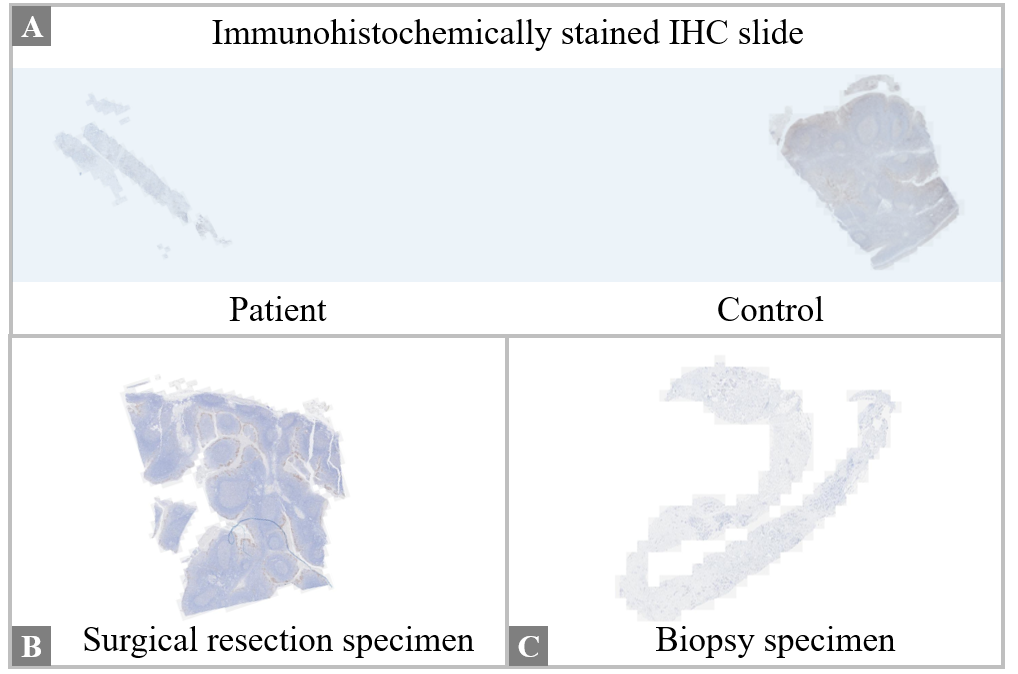
\includegraphics[width=1.0\columnwidth]{figs/IHC.png}
    \caption{Example of source images: (A) Immunohistochemically stained IHC slide, (B) Surgical resection specimen, and (C) Biopsy specimen.}
    \label{fig:IHC}
\end{figure}

\section{Research Background and Motivation}
 % 本研究来源于我们与多位癌症病理领域专家的合作与讨论。我们的合作对象包括两位病理科临床医生，他们长期专注于多种癌症病理诊断和预后分析等；同时包括两位病理图像解析专家，他们长期专注于数字病理图像分析、全切片图像建模、组织与细胞级识别及智能分析方法研究。在临床病理研究中，专家通常对IHC切片进行染色，通过颜色评估PD-L1表达情况，即组织的癌变情况。如图Xa所示为一张临床使用的IHC切片的示意图，长和宽是临床玻片的实际形态，其左右两侧分散多个病理组织，中间呈现大面积的空白。玻片的一侧为患者待测样本，另一侧为对照组织。使用对照组的目的并非与患者样本直接进行差异对比，而是用于判断免疫组化染色是否正常、抗体定位是否准确以及阳性表达是否可靠，从而排除由 IHC 染色灵敏度不足导致的假阴性。通常对照组并非全是健康组织，其亦会是癌变阳性的组织。在染色达标后，医生通过对患者组织的颜色占比进行肉眼评估，以 5%、10%、20% 、50%等若干整十数区间进行粗略描述，以衡量癌变的严重程度，进而辅助评估是否可以对患者用药。然而，由于患者组织的采样方式不同，呈现为多种形态，例如，手术切除样本（如图Xb），通常呈现为块状；穿刺活检样本（如图Xc），通常呈现为细长条状，其在包埋和切片过程中可能被分成多段，分布在玻片的不同位置。医生对IHC切片的评估需要通过肉眼定位到肿瘤区域，再通过放缩观察和核验，这种方式受制于病理组织的形态，穿刺活检样本形态弯曲多变且存在包埋和多段的情况，难以衡量其PD-L1 阳性表达占比，不同医生之间经常存在较大的判读差异。因此，TPS被提出以精确衡量样本的阳性占比，然而此，一方面，患者组织与对照组织在切片中的左右位置并不完全固定，且形态各异，需要专家结合具体的玻片进行细致判断，另一方面，虽然现有工具能够对全片IHC进行TPS评估，单一的TPS评分不足以精确衡量组织癌变情况。此外，IHC切片中可能存在坏死组织、弱阳性表达、肿瘤与非肿瘤细胞混杂等，都会影响最终评分的稳定性和可信度。整体上，IHC切片呈现为组织分布离散、空白区域较多、患者组织与对照组织共存、活检与手术样本形态差异明显等特点，现阶段缺少对全片进行多层级追溯分析与细节评估的交互式可视分析系统，从而提高 PD-L1表达的临床判读效率、稳定性和可信度。
This study was motivated by our collaboration and discussions with several experts in cancer pathology. Our collaborators include a clinical pathologist who have long been engaged in the pathological diagnosis and prognostic assessment of various cancers, as well as a pathology image analysis expert whose research focuses on digital pathology image analysis, whole-slide image modeling, tissue- and cell-level recognition, and intelligent analysis methods. In clinical pathology practice, experts usually assess PD-L1 expression on immunohistochemically stained slides according to the staining appearance, thereby evaluating the pathological status of the tissue. Fig.~\ref{fig:IHC}A shows a schematic example of a clinically used IHC slide. The length and width follow the actual configuration of a clinical glass slide, with multiple tissue fragments distributed on the left and right sides and a large blank area in the middle. One side of the slide contains the patient specimen to be assessed, while the other side contains control tissue. The purpose of the control tissue is not to conduct a direct differential comparison with the patient specimen, but to determine whether the IHC staining is adequate, whether the antibody localization is accurate, and whether positive expression can be reliably detected, thereby excluding false-negative results caused by insufficient staining sensitivity. In general, the control tissue is not necessarily normal tissue; it may also be known tumor-positive tissue.

After the staining quality is confirmed, pathologists visually estimate the proportion of stained regions in the patient tissue and describe the result using coarse percentage intervals, such as 5\%, 10\%, 20\%, and 50\%, to characterize the severity of tumor-related expression and support treatment decision-making. However, patient specimens can present diverse morphologies due to different sampling procedures. For example, surgical resection specimens, as shown in Fig.~\ref{fig:IHC}B, usually appear as tissue blocks, whereas needle biopsy specimens, as shown in Fig.~\ref{fig:IHC}C, often appear as elongated strips. During embedding and sectioning, biopsy tissues may be divided into multiple fragments and distributed across different positions on the slide. The assessment of IHC slides requires pathologists to first visually locate tumor regions and then verify them through zooming and close inspection. This process is strongly affected by the morphology of pathological tissue. In particular, needle biopsy specimens are often curved, irregular, and fragmented after embedding and sectioning, making it difficult to estimate the proportion of PD-L1-positive expression. As a result, considerable inter-observer variability may occur among different pathologists. Therefore, TPS has been introduced to more precisely quantify the positive proportion of the specimen. Nevertheless, several challenges remain. On the one hand, the relative positions of the patient specimen and the control tissue on the slide are not fixed, and their morphologies vary substantially, requiring experts to make careful judgments based on each individual slide. On the other hand, although existing tools can perform TPS assessment on whole-slide IHC images, a single TPS value is insufficient to fully characterize the pathological status of the tissue. In addition, necrotic tissue, weak positive expression, and the mixture of tumor and non-tumor cells in IHC slides can all affect the stability and reliability of the final score. 

IHC slides are characterized by dispersed tissue distributions, large blank regions, the coexistence of patient specimens and control tissues, and substantial morphological differences between biopsy and surgical specimens. At present, there remains a lack of interactive visual analytics systems that support multi-level evidence tracing and detailed assessment across whole-slide images, which is essential for improving the efficiency, stability, and reliability of clinical PD-L1 expression interpretation.

% 本文面向肺癌 PD-L1 表达的临床分析，主要包含以下四个关键设计目标：
% DG1：多层级识别
% PD-L1 预后评估不仅需要从整体上判断切片中阳性与阴性表达区域的分布情况，还需要在细胞层面对膜染色状态进行精细识别，以支持更可靠的阳性/阴性判定。然而，医生无法对超大尺寸的图片进行详尽的标注，高成本细胞标注和显式分割流程也限制了其在大规模推理中的应用。因此，需要在区域级与细胞级的图像上进行快速状态识别，实现对 PD-L1 表达状态的准确识别与高可信判断。
% DG2：多尺度可视化PD-L1 IHC 切片具有显著的多尺度特征，全图和区域级的图像可以观察宏观的染色表达分布，细胞级图像则有助于识别细胞膜染色、局部异质区域和细胞边界细节。在临床阅片过程中，医生需要先找到肿瘤区域，再进行相关指标的分析。在不同尺度图片进行切换分析，有助于医生进行全局筛查与局部确认验证。因此，系统需要提供区域级与细胞级同步联动的多尺度可视化机制，以支持高效观察。
% DG3：自动量化分析医生通常需要对感兴趣的区域进行重点观察，选择和自动分析感兴趣区域的免疫表达有助于快速精细化评估肿瘤状态。然而，由于组织异质性、肿瘤细胞与非肿瘤细胞混杂、染色强度波动以及弱阳性边界样本难以区分等，TPS计算评估面临噪声干扰、跨尺度建模困难和可解释性不足等挑战。因此，系统需要对组织成分及相关表达指标进行自动计算与统计分析，从而提高评估过程的客观性和结果的可解释性。
% DG4：高效交互探索PD-L1 全切片图像通常规模大、信息密集，专家需要在复杂组织区域中不断定位感兴趣区域、筛选关键信息并比较不同层级的分析结果，这一过程耗时且容易产生视觉负担，尤其在弱染色区域、细胞密集区域以及异质性显著区域。因此，系统需要提供高效的交互探索能力，支持快速导航、灵活筛选、结果联动和按需细查，从而提升评估的整体效率。

\section{Design Goals}
We focus on the clinical analysis of PD-L1 expression in lung cancer and define the following four key design goals:

\textbf{DG1: Multi-level Recognition.}
PD-L1 prognostic assessment requires not only an overall judgment of the distribution of positive and negative expression regions on a slide, but also fine-grained identification of membranous staining status at the cellular level, so as to support more reliable positive/negative determination. However, physicians cannot provide detailed annotations for ultra-large images, and the high cost of cell-level annotation and explicit segmentation workflows also limits their application in large-scale inference. Therefore, rapid state recognition at both the region and cell levels is required to achieve accurate identification and high-confidence assessment of PD-L1 expression status.

\textbf{DG2: Multi-scale Visualization.}
PD-L1 IHC slides exhibit prominent multi-scale characteristics. Whole-slide and region-level images enable the observation of macroscopic staining and expression distributions, whereas cell-level images help identify cell membrane staining, local heterogeneous regions, and cell boundary details. In clinical slide reading, physicians need to first locate tumor regions before analyzing relevant indicators. Switching between images at different scales helps physicians perform global screening and local confirmation. Therefore, the system needs to provide a multi-scale visualization mechanism with synchronized coordination between region-level and cell-level views to support efficient observation.

\textbf{DG3: Automated Quantitative Analysis.}
Physicians usually need to focus on regions of interest, and selecting and automatically analyzing the immune expression within these regions can facilitate rapid and refined assessment of tumor status. However, due to tissue heterogeneity, the mixture of tumor and non-tumor cells, variations in staining intensity, and the difficulty of distinguishing weakly positive borderline cases, TPS calculation and assessment face challenges such as noise interference, cross-scale modeling difficulty, and insufficient interpretability. Therefore, the system needs to automatically compute and statistically analyze tissue components and related expression indicators, thereby improving the objectivity of the assessment process and the interpretability of the results.

\textbf{DG4: Efficient Interactive Exploration.}
PD-L1 whole-slide images are typically large in scale and information-dense. Experts need to continuously locate regions of interest, filter key information, and compare analysis results across different levels within complex tissue regions. This process is time-consuming and prone to visual burden, especially in weakly stained regions, densely cellular regions, and highly heterogeneous regions. Therefore, the system needs to provide efficient interactive exploration capabilities, supporting rapid navigation, flexible filtering, coordinated result exploration, and on-demand detailed inspection, thereby improving the overall efficiency of the assessment.


\begin{figure*}
    \centering
    \includegraphics[width=1.0\textwidth]{figs/Workflow.png}
    \caption{The visual analytics pipeline of our PD-L1 expression evaluation system is composed of multi-level representation modeling, patch-level quantitative analysis, and cell-level interactive exploration stages.}
    \label{fig:workflow}
\end{figure*}


\section{Data Description}
% \subsection{Data Acquisition}
%本研究所采用的数据集包含 20 张肺癌 PD-L1 免疫组织化学（IHC）全视野切片。这些切片在扫描后，其 level0 图像尺寸平均约为 73,340×37,700 像素。在 level0 下以 512×512 进行切块并剔除空白区域后，共得到 63,194 张 IHC patch。该数据集不仅涵盖了手术切除的大块组织样本，还包含了临床中更为复杂、形态细长且易断裂的穿刺活检样本，能够充分验证系统在不同组织形态、异质性分布以及不同 PD-L1 表达丰度下的稳健性与实用性。其包含的像素量达数亿级，体现了数字病理数据典型的超高分辨率与多尺度特征。

The dataset used in this study comprises 20 PD-L1 IHC whole-slide images of lung cancer. After scanning, the level-0 images have an average size of approximately $73{,}340 \times 37{,}700$ pixels. By tiling at level 0 with a patch size of $512 \times 512$ pixels and filtering out empty background regions, we obtained a total of 63{,}194 IHC patches. The dataset covers not only large surgical resection specimens but also the clinically more challenging needle biopsy specimens, which are typically thin, elongated, and prone to fragmentation. It therefore spans diverse tissue morphologies, heterogeneous spatial distributions, and varying levels of PD-L1 expression, enabling a thorough evaluation of the robustness and practical utility of the system. With a total pixel count reaching the hundred-million scale, the dataset exemplifies the typical ultra-high resolution and multi-scale characteristics of digital pathology data.


\section{METHODS}
\subsection{Overall Workflow}
%如图 X 所示，我们系统的整体工作流程包括多层级表达建模、自动量化分析以及交互式可视判读。在第一阶段，系统首先将高分辨率全切片图像解构为 512*512 像素的网格片段，并利用细胞感知的弱监督蒸馏框架并行执行 Patch 级的 TPS 分级与细胞级的状态识别。在第二阶段，系统通过空间索引技术自动过滤无效的空白背景，并根据临床阈值对有效肿瘤区域的 Patch 进行 TPS 指标的自动分档计算与统计。在第三阶段，系统提供多尺度联动的交互界面，通过 ROI 选区与细胞级详情卡片，并借助Agent 辅助医生进行病灶定位与细节追溯，从而提升 PD-L1 评估的一致性与可解释性。
As shown in Fig.~\ref{fig:workflow}, the overall workflow of the system comprises multi-level expression modeling, automated quantitative analysis, and interactive visual interpretation. In Phase~I, high-resolution whole-slide images are decomposed into pixel patches, and a cell-aware weakly supervised distillation framework performs patch-level TPS grading and cell-level state recognition in parallel. In Phase~II, the system uses spatial indexing to automatically filter invalid blank backgrounds and, based on clinical thresholds, performs automatic bin-wise computation and statistical aggregation of TPS indicators over patches within valid tumor regions. In Phase~III, the system provides a multi-scale coordinated interactive interface that, through region of interest (ROI) selection and cell-level detail cards, along with an agent to assist pathologists in lesion localization and evidence tracing, thereby enhancing the consistency and interpretability of PD-L1 assessment.

%\subsection{基于知识蒸馏与双任务 Transformer 的 PD-L1 表达识别}
% \subsection{PD-L1 Expression Recognition via Knowledge Distillation and Dual-task Transformer}
\subsection{PD-L1 Expression Status Classification}

%本文所依托的算法是一种面向 PD-L1 IHC 图像 TPS 自动评估的细胞感知弱监督建模方法。其核心目标是在不依赖人工逐细胞精细标注和推理阶段完整实例分割的前提下，从病理图像中提取与 TPS 判读相关的细胞级证据，并进一步完成 patch-level 的 TPS 分级。算法首先在训练阶段利用细胞实例掩码和病理预训练模型构建教师端细胞表征。具体而言，设教师网络提取的特征图为 $F^T$，第 $i$ 个细胞实例在特征图坐标系下对应的掩码区域为 $\tilde{M}_i$，则该细胞的 teacher 表征可通过掩码区域内的特征平均池化得到：$$z_i^T = \frac{1}{|\tilde{M}_i|} \sum_{(u,v)\in \tilde{M}_i} F^T(u,v)$$其中，$z_i^T$ 表示第 $i$ 个细胞的教师端特征向量，$(u,v)$ 表示特征图上的空间坐标，$F^T(u,v)$ 表示教师特征图在该位置的特征向量，$|\tilde{M}_i|$ 表示该细胞掩码区域内的特征点数量。随后，算法通过蒸馏将多阶段细胞特征提取过程压缩到轻量学生网络中；并使用点监督定位头预测细胞中心，基于预测细胞位置采样细胞级特征。在下游预测阶段，算法将一个 patch 内的细胞特征组织为变长序列，输入共享编码器的双任务 Transformer。模型包含两个输出分支：细胞级分支用于预测肿瘤候选细胞的 PD-L1 阴性/阳性状态，patch 级分支用于预测该图像块对应的 TPS 分级。与直接基于阳性细胞比例进行阈值统计的方法不同，该算法通过 Transformer 建模细胞间关系、空间上下文和整体染色分布，并通过跨尺度一致性约束对齐细胞级阳性比例与 patch-level TPS 预测。整体训练目标可概括为：$$\mathcal{L} = \mathcal{L}_{cell} + \mathcal{L}_{patch} + \lambda_{cons}\mathcal{L}_{cons}, \quad \mathcal{L}_{cons} = \left| \hat{t} - \frac{1}{N}\sum_{i=1}^{N} p_i \right|$$其中，$\mathcal{L}_{cell}$ 表示细胞级 PD-L1 阴性/阳性判别损失，$\mathcal{L}_{patch}$ 表示 patch-level TPS 监督损失，$\mathcal{L}_{cons}$ 表示跨尺度一致性损失，$\lambda_{cons}$ 为一致性损失权重；$\hat{t}$ 表示 patch 分支预测的 TPS 估计值，$p_i$ 表示第 $i$ 个细胞由细胞级分支输出的阳性概率，$N$ 表示该 patch 内的细胞候选数量。这里的一致性损失使用 $L_1$ 距离，约束 patch-level TPS 估计值与细胞级阳性比例估计值保持一致。最终，模型在一次前向推理中即可同时输出细胞位置、细胞级 PD-L1 状态和 patch-level TPS 分类结果。实验结果表明，该方法相比传统 DAB 阈值、手工特征、通用 IHC 量化工具和公开 PD-L1 pipeline，在 patch-level TPS 四分类任务上具有更稳定的表现；同时在完成 TPS 分级的同时，保留与病理判读过程对应的细胞级证据。
The algorithm underlying our system is a cell-aware weakly supervised modeling method for automatic TPS assessment on PD-L1 IHC images. Its core objective is to extract TPS-related cell-level evidence from pathology images and to further perform patch-level TPS grading, without requiring manual per-cell annotation during training or full instance segmentation at inference time.

In the training stage, the algorithm first leverages cell instance masks together with a pathology pre-trained model to construct teacher-side cell representations. Specifically, let $F^T$ denote the feature map extracted by the teacher network, and let $\tilde{M}_i$ denote the mask region of the $i$-th cell instance in the feature-map coordinate system. The teacher representation of this cell is then obtained by average pooling of the features within the mask region:
$$z_i^T = \frac{1}{|\tilde{M}_i|} \sum_{(u,v)\in \tilde{M}_i} F^T(u,v),$$
where $z_i^T$ denotes the teacher-side feature vector of the $i$-th cell, $(u,v)$ denotes a spatial coordinate on the feature map, $F^T(u,v)$ denotes the teacher feature vector at that location, and $|\tilde{M}_i|$ denotes the number of feature points inside the cell mask. Subsequently, the algorithm distills this multi-stage cell feature extraction process into a lightweight student network, and uses a point-supervised localization head to predict cell centers, based on which cell-level features are sampled at the predicted cell positions.

In the downstream prediction stage, the cell features within a patch are organized as a variable-length sequence and fed into a dual-task Transformer with a shared encoder. The model has two output branches: the cell-level branch predicts the PD-L1 negative/positive status of candidate tumor cells, while the patch-level branch predicts the corresponding TPS grade of the patch. Unlike methods that directly apply a threshold over the proportion of positive cells, the proposed algorithm uses the Transformer to model inter-cell relations, spatial context, and the overall staining distribution, and employs a cross-scale consistency constraint to align the cell-level positive ratio with the patch-level TPS prediction. The overall training objective is:
$$\mathcal{L} = \mathcal{L}_{cell} + \mathcal{L}_{patch} + \lambda_{cons}\mathcal{L}_{cons}, \quad \mathcal{L}_{cons} = \left| \hat{t} - \frac{1}{N}\sum_{i=1}^{N} p_i \right|,$$
where $\mathcal{L}_{cell}$ is the cell-level PD-L1 negative/positive discrimination loss, $\mathcal{L}_{patch}$ is the patch-level TPS supervision loss, $\mathcal{L}_{cons}$ is the cross-scale consistency loss, and $\lambda_{cons}$ is the corresponding weight. $\hat{t}$ denotes the TPS estimate predicted by the patch branch, $p_i$ denotes the positive probability of the $i$-th cell predicted by the cell branch, and $N$ denotes the number of cell candidates within the patch. The consistency loss uses the $L_1$ distance to enforce agreement between the patch-level TPS estimate and the cell-level positive-ratio estimate. As a result, in a single forward pass the model simultaneously outputs cell locations, cell-level PD-L1 states, and patch-level TPS classification results. Experimental results show that, compared with traditional DAB-threshold methods, hand-crafted features, general-purpose IHC quantification tools, and open-source PD-L1 pipelines, the proposed method achieves more stable performance on the four-class patch-level TPS task, while preserving cell-level evidence that is directly aligned with the pathological interpretation process.


\subsection{Visual Design and Interaction}

\subsubsection{Data Selection View}

%左侧栏（如图1A,B）的核心设计目标是提供高效的数据入口，避免用户在海量数据中进行盲目搜索。该模块由上下两部分组成：
%specimen explorer： 在数据导入阶段，系统从服务端解析全切片图像的金字塔清单，并在左上角生成病例卡片。为了提升临床筛查效率，系统在客户端默认按平均 TPS 评分对病例进行降序排列，并通过状态短语（如 High PD-L1, Elevated, Low expressors）与高对比度边框进行视觉编码(如图A)，使高表达风险病例脱颖而出。
%patche gallery： 位于左栏下半部(如图1B)的patche gallery是连接宏观与微观的检索枢纽。系统首先过滤掉无细胞级数据的背景图像块，仅保留有效肿瘤区域。图库内置了基于临床评分标准的分档筛选器。当用户在图库中单击特定高风险 Patch 时，系统将触发飞行定位交互，驱动主视图瞬间平移缩放至该空间位置。此外patche gallery与中栏的ROI selection保持深度联动：令全片有效 Patch 集合为 P，当前选区为 ROI，图库仅渲染属于 P∩ROI 的交集图像块，并按预测 TPS 值（τ）动态重排。
The core design goal of the left sidebar (Fig.~\ref{fig:teaser}A,~B) is to provide an efficient entry point into the data and to prevent users from searching blindly through a large case pool. This module is composed of two vertically stacked components.

\textbf{Specimen Explorer.} During the data import stage, the system parses the image-pyramid manifest of each whole-slide image on the server side and generates case cards in the upper-left panel. To improve clinical screening efficiency, cases are by default sorted in descending order by their average TPS scores on the client side, and are visually encoded with status phrases (e.g., \textit{High PD-L1}, \textit{Elevated}, \textit{Low expressors}) and high-contrast borders (Fig.~\ref{fig:teaser}A), so that high-expression cases stand out at a glance.

\textbf{Patch Gallery.} Located in the lower half of the left column (Fig.~\ref{fig:teaser}B), the Patch Gallery serves as a retrieval hub bridging macroscopic and microscopic scales. The system first filters out background patches that contain no cell-level data and retains only valid tumor regions. The gallery is equipped with a built-in bin-wise filter based on clinical scoring standards. When the user clicks on a specific high-risk patch, the system triggers a fly-to interaction that smoothly pans and zooms the main view to the corresponding spatial location. In addition, the Patch Gallery maintains a tight linkage with the ROI selection in the central panel: let the set of valid patches on the whole slide be $P$ and the current selection be $\mathrm{ROI}$; the gallery only renders the intersection $P \cap \mathrm{ROI}$ and dynamically reorders these patches according to their predicted TPS value $\tau$.


\subsubsection{IHC Image View and TPS Distribution View}

%中栏（如图1C,D）是系统的核心阅片与量化分析枢纽，占据了最大的屏幕空间，旨在解决超大分辨率图像在导航中的空间迷失痛点与异质性量化难题。
%IHC Image View： 上半部分基于 OpenSeadragon 构建了平滑的图像金字塔渲染引擎(如图C)。为了在不阻挡底层组织形态的前提下提供视觉捷径，系统利用核密度估计在 WSI 表面叠加了一层高亮度的 TPS 热力图。此外，用户可通过局部 ROI 工具在画面上框选感兴趣的肿瘤微环境。系统底层算法会自动将用户绘制的矩形吸附对齐至 $512 \times 512$ 像素的 Patch 网格，并实时提取空间交集内的特征数据。
%TPS Distribution View： 中栏下半部分设计了高度定制化的 TPS 定量仪表盘(如图D)，通过TPS Distribution View、Selection ROI实现多维数据表征。对于模型输出的每个 Patch 的预测得分 $\tau \in [0, 1]$，系统将其映射为细粒度的 $0.1\%$ 直方图分箱：$$k = \text{clamp}(\text{round}(1000 \cdot \tau), 0, 1000)$$为使直方图的视觉分布完美契合病理四大临床阈值，系统在横轴（X 轴）引入了基于数据密度的比例尺映射。记临床档位 $b \in \{\text{Neg, T1, T10, T50}\}$ 中的 Patch 数量为 $n_b$，总 Patch 数为 $N_{\text{tot}}$，则各临床档位在绘图区总宽度 $W_{\text{plot}}$ 中分配的像素带宽 $W_b$ 为：$$W_b = \begin{cases} \frac{n_b}{N_{\text{tot}}} W_{\text{plot}}, & N_{\text{tot}} > 0 \\ \frac{1}{4} W_{\text{plot}}, & N_{\text{tot}} = 0 \end{cases}$$该映射保证了直方图每个背景带内柱子的“总质量”精确等于该档位的 Patch 真实占比。同时，为防止局部极值导致直方图垂直方向的视觉饱和，系统引入了动态填充比 $\rho$（全片模式 $\rho = 0.9$，ROI 模式 $\rho = 0.8$）来计算 Y 轴的显示上界：$$Y_{\max} = \frac{\tilde{c}_{\max}}{\rho}$$在此仪表盘中，用户可以通过观察直方图是否呈现双峰结构来敏锐地捕捉肿瘤微环境的空间异质性特征。
The central panel (Fig.~\ref{fig:teaser}C,~D) occupies the largest amount of screen space and serves as the core slide-reading and quantitative-analysis hub of the system. It is designed to address two key pain points encountered when navigating ultra-high-resolution images: spatial disorientation and the difficulty of quantifying heterogeneity.

\textbf{IHC Image View.} The upper part of the central panel builds a smooth image-pyramid rendering engine based on OpenSeadragon (Fig.~\ref{fig:teaser}C). To provide visual shortcuts without occluding the underlying tissue morphology, the system uses kernel density estimation to overlay a high-contrast TPS heatmap on the WSI surface. In addition, users can frame regions of interest in the tumor microenvironment using a local ROI tool. The underlying algorithm automatically snaps the user-drawn rectangle to the $512 \times 512$ pixel patch grid and extracts feature data within the spatial intersection in real time.

\textbf{TPS Distribution View.} The lower part of the central panel provides a highly customized TPS quantitative dashboard (Fig.~\ref{fig:teaser}D). Through the TPS distribution histogram and the selection-linked summary statistics, it enables multi-dimensional data characterization. For each patch with predicted TPS score $\tau \in [0, 1]$ output by the model, the system maps it to a fine-grained $0.1\%$ histogram bin:
$$k = \mathrm{clamp}(\mathrm{round}(1000 \cdot \tau), 0, 1000).$$
To make the visual distribution of the histogram align with the four clinical TPS thresholds, the system introduces a density-aware scale mapping on the horizontal axis. Let $n_b$ be the number of patches in clinical bin $b \in \{\mathrm{Neg}, \mathrm{T1}, \mathrm{T10}, \mathrm{T50}\}$, and let $N_{\mathrm{tot}}$ be the total number of valid patches. The pixel width $W_b$ allocated to each clinical bin within the total plotting width $W_{\mathrm{plot}}$ is given by:
$$W_b = \begin{cases} \dfrac{n_b}{N_{\mathrm{tot}}} W_{\mathrm{plot}}, & N_{\mathrm{tot}} > 0, \\[4pt] \dfrac{1}{4} W_{\mathrm{plot}}, & N_{\mathrm{tot}} = 0. \end{cases}$$
This mapping ensures that the total mass of the histogram bars within each background band exactly matches the true proportion of patches in the corresponding clinical bin. To prevent local extremes from causing visual saturation along the vertical axis, the system further introduces a dynamic filling ratio $\rho$ (whole-slide mode: $\rho = 0.9$; ROI mode: $\rho = 0.8$) to determine the upper bound of the Y axis:
$$Y_{\max} = \frac{\tilde{c}_{\max}}{\rho}.$$
With this dashboard, users can sensitively detect the spatial heterogeneity of the tumor microenvironment by examining whether the histogram exhibits a bimodal structure.


\begin{figure*}
    \centering
    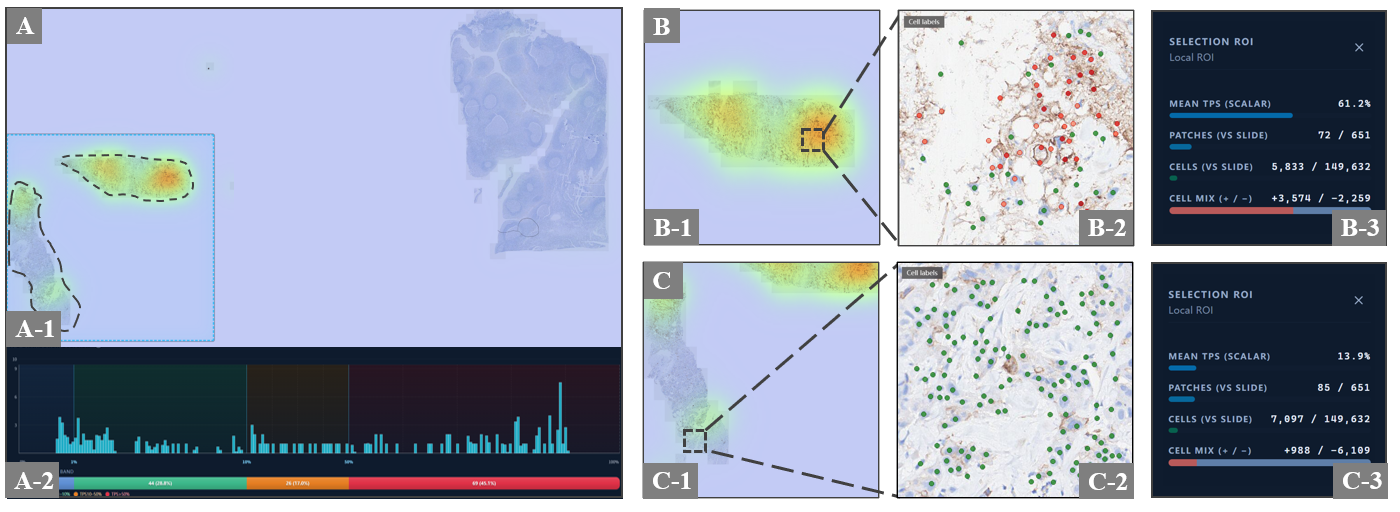
\includegraphics[width=1.0\textwidth]{figs/case1.png}
    \caption{Assessment of Biopsy Heterogeneity: (A) Global Overview View, (B) High-expression Region (Strip A), (C) Low-expression Region (Strip B) }
    \label{fig:case1}
\end{figure*}

\subsubsection{Cell-Level View}

%右侧栏（如图1E）的目的是打破算法的黑盒特性，提供坚实的底层数据解释支持，从而帮助医生建立对量化评分的信任。
%多图层预览带： 当主视图平滑导航至目标斑块时，右上角的预览模块将自动同步加载该区域的高分辨率图像(如1图E)。该组件集成了细胞阴阳分类图（Cell Types）(如图1E-1)与细胞概率热力图（Cell Probability）(如图1E-2)，并支持在微型视口内进行独立的缩放与平移操作。两类图层保持像素级的实时联动，允许专家在不干扰主视口全局上下文的情况下，对局部病灶进行多维度细节核查，有效缓解了图层频繁切换带来的认知损耗。
%Selected patch： 预览带下方是一个富信息统计面板(如图1E-3)。该面板通过异步请求实时加载当前 Patch 内部所有细胞的精确坐标与分类概率。面板利用堆叠条形图直观对比阴性与阳性肿瘤细胞的绝对计数，并计算局部的细胞加权 TPS 百分比。更重要的是，它同时展示了当前 Patch 的细胞基数在全片细胞总基数中的权重贡献比例。这种将“微观表达强度”与“宏观成分权重”并列展示的策略，构成了完整的证据追溯链条，有效修正了因局部高表达造成的视觉偏差。
The right sidebar (Fig.~\ref{fig:teaser}E) is designed to open up the black box of the algorithm and to provide solid underlying data-interpretation support, thereby helping pathologists build trust in the quantitative scoring.

\textbf{Multi-layer Preview Strip.} When the main view smoothly navigates to a target patch, the preview module in the upper-right corner automatically and synchronously loads the high-resolution image of that region (Fig.~\ref{fig:teaser}E). This component integrates the cell tpye map (\textit{Cell labels}, Fig.~\ref{fig:teaser}E-1) and the cell probability map (\textit{P(cell) map}, Fig.~\ref{fig:teaser}E-2), and supports independent zooming and panning within the mini-viewport. The two layers are linked at the pixel level in real time, allowing experts to perform multi-dimensional detailed verification of local lesions without disturbing the global context of the main viewport, thereby alleviating the cognitive load caused by frequent layer switching.

\textbf{Cell-Level Detail Card (Selected Patch).} Below the preview strip lies an information-rich statistical panel (Fig.~\ref{fig:teaser}E-3). This panel asynchronously loads the precise coordinates and classification probabilities of all cells within the current patch in real time. It uses stacked bar charts to intuitively compare the absolute counts of negative and positive tumor cells, and computes the local cell-weighted TPS. More importantly, it also displays the weight contribution of the cell base of the current patch relative to the total cell base of the whole slide. By juxtaposing ``microscopic expression intensity'' and ``macroscopic component weight'', this design forms a complete chain of evidence tracing and effectively corrects the visual bias caused by local high expression.


\subsubsection{Pathology Insight Agent}

%为提升系统的信息获取效率与医学解释性，系统引入 Pathology Insight Agent (如图F)作为统一的自然语言问答层，主要用于辅助医生理解复杂的量化指标与空间异质性特征。在整体架构设计上，系统明确剥离了复杂的交互编排与报告生成功能，采用“外层语义解析+内层受控检索”的轻量级分层策略。
%在外层，系统接入通用大语言模型作为自然语言解析模块，当前实现采用 DeepSeek 模型对用户的请求进行语义理解与意图识别，并将其精准映射为当前病例、微观图像块、局部空间选区以及临床细胞阴阳性阈值等结构化上下文参数。
%在内层，为了保障医疗场景的严谨性并彻底杜绝大模型的“幻觉”问题，Agent 被严格限制了系统操作与调度权限，其核心职能仅聚焦于基于事实的客观问答。当完成请求映射后，系统通过受控的数据接口，直接向底层数据库与后台计算服务发起检索，获取如全片最高 TPS 图像块、局部 ROI 与全局细胞计数对比等唯一的原始统计快照。
%用户可以与 Agent 进行对话问答，但是需要特别说明的是，为了确保医学决策的安全性，我们预定义了一系列病理专家在临床阅片时可能高度关注的核心问题，并给出了预先计算的客观数据结果。系统的回答建立在这些唯一客观的预计算数值之上，通过读取结构化输出字段，并结合固定的文本模板完成填空式组织。系统所输出的病理洞察仅仅是对分析管线底层数值的规范化复述，而不是由大语言模型自由生成科学诊断结论，也不是通过视觉大模型识别图像内容后再进行主观推断，从而在提供灵活问答体验的同时，最大程度地保障了辅助判读的安全边界。
To improve the information-access efficiency and medical interpretability of the system, we introduce the \textit{Pathology Insight Agent} (Fig.~\ref{fig:teaser}F) as a unified natural-language question-answering layer, mainly designed to help pathologists understand complex quantitative indicators and spatial heterogeneity features. At the architectural level, we deliberately decouple complex interaction orchestration and free-form report generation, and adopt a lightweight hierarchical strategy of ``outer-layer semantic parsing plus inner-layer controlled retrieval.''

At the outer layer, a general-purpose large language model is integrated as the natural-language parsing module. The current implementation uses the DeepSeek model to perform semantic understanding and intent recognition on user queries, and to map them precisely into structured context parameters such as the current case, the patch under inspection, the local ROI selection, and the clinical thresholds for cell-level positivity.

At the inner layer, to ensure rigor in medical scenarios and to fundamentally eliminate hallucinations from the large language model, the agent is strictly constrained in terms of system-operation and orchestration permissions. Its core function is limited to fact-based objective question-answering. After completing the request mapping, the system issues queries to the underlying database and back-end computation services through controlled data interfaces, retrieving unique raw statistical snapshots such as the patch with the highest TPS on the entire slide or the comparison between the cell counts within the local ROI and those across the whole slide.

Users can engage in conversational question-answering with the agent. It should be emphasized that, in order to ensure the safety of medical decision-making, we pre-define a set of core questions that pathologists are likely to focus on during clinical reading, together with their pre-computed objective answers. The system's responses are built on top of these unique, objective, pre-computed values: the agent reads structured output fields and uses fixed textual templates to organize the final answer in a fill-in-the-blank manner. The pathology insights produced by the system are thus standardized restatements of the underlying numerical results from the analysis pipeline, rather than free-form scientific diagnostic conclusions generated by the language model or subjective inferences drawn from a vision-language model's interpretation of the image content. This design provides a flexible conversational experience while preserving a clear safety boundary for assisted interpretation.



\begin{figure*}[t]
    \centering
    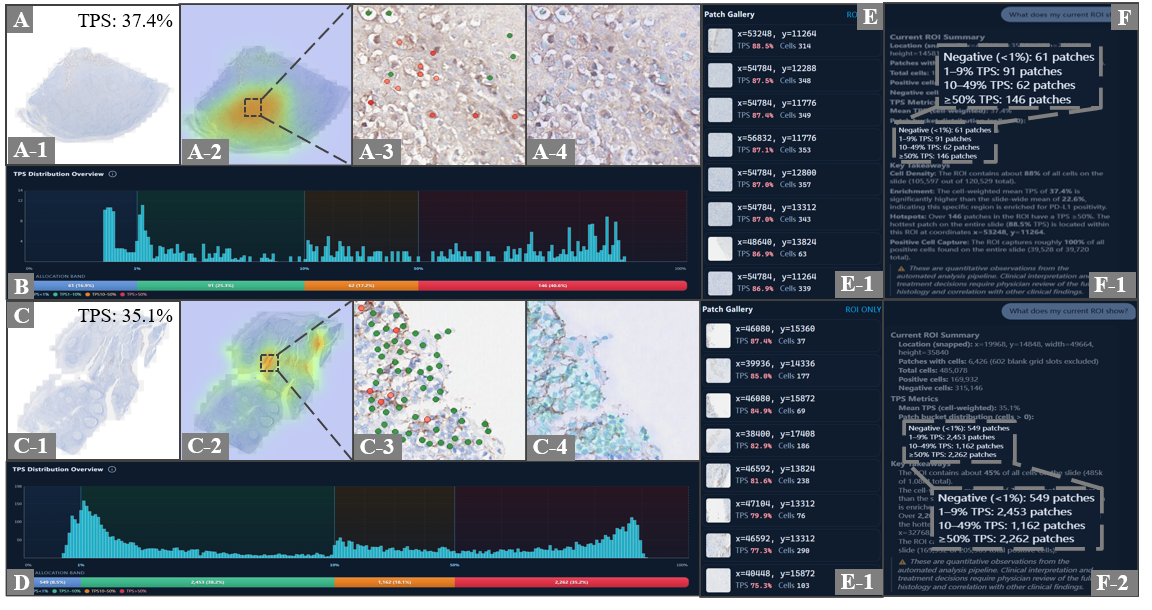
\includegraphics[width=1.0\textwidth]{figs/case2.png}
    \caption{Comparative Analysis of Boundary Cases:(A, C) pathology insights, (B, D) TPS Distribution Overview,(E)Patch Gallery, (F) Pathology Insight Agent}
    \label{fig:case2}
\end{figure*}

\section{Case Studies}

%为了评估系统在肺癌 PD-L1 临床判读中的有效性，我们利用 20 张真实IHC全视野切片开展了案例研究，重点考察系统在多层级证据追溯、空间异质性分析以及辅助科研假设生成中的支持能力。案例评估由两位合作领域专家共同参与：一位是具有十余年临床经验的病理主任医师（E1），另一位是专注于计算病理学的学术研究员（E2）。他们从临床工作流适配性、结果一致性、交互效率及系统可解释性等多个维度进行了实操反馈与评价。
To evaluate the effectiveness of the system in the clinical interpretation of lung cancer PD-L1, we conducted case studies on 20 real IHC whole-slide images, focusing on the system's ability to support multi-level evidence tracing, spatial heterogeneity analysis, and assisted research hypothesis generation. The case evaluation involved two collaborating domain experts: E1 is a chief pathologist with more than ten years of clinical experience, and E2 is an academic researcher specializing in computational pathology. They provided hands-on feedback and evaluations from multiple dimensions, including clinical workflow adaptability, result consistency, interaction efficiency, and system interpretability.



%\subsection{Case1: 穿刺样本异质性评估}
\subsection{Case1: Assessment of Biopsy Heterogeneity}

%PD-L1 表达在肿瘤微环境中常呈现高度的空间异质性，同一活检组织内可能并存极低与极高表达的病灶。若仅采用全局聚合指标，往往会掩盖具有临床意义的局部危险区域。这种异质性在穿刺小标本中尤为关键，因为有限的取样量极易受“取到哪一块”的影响，从而产生显著的判读误差风险。本案例构造了一类典型的临床干扰场景：左侧为患者穿刺，右侧为对照（如图4A-1）。由于患者侧的穿刺组织沿扫描方向过长，在物理制片与网格划分时被切断为两块相邻的区域（Strip A 与 Strip B）。全局统计显示，患者侧的总体 TPS 处于 35.7% 的关键边界区间，但局部的表达却发生极度分化：一块高达 61.2%，另一块仅为 13.9%。
%在分析初始，系统底部的 TPS 分布总览 提供了全局的数据线索。该视图给出了 0.1% 细粒度 Bin 聚合后经比例尺映射的直方图，并与临床四档背景带严格对齐；同时，全片的 TPS 分配带 宏观呈现了各档位的混合比例。 在此视图中（如图4A-2），直方图呈现出典型的双峰结构——一个主峰集中在 1% 附近的极低表达区，另一个次峰则出现在 50%−100% 的高表达区间。这种反常的形态分布构成了关键的可视化线索，引导分析逻辑转向热力图的空间拆解。通过本系统提供的热力图进行细粒度空间分析，可以直观观察到显著的拓扑差异：左侧的两块组织表现出截然不同的着色特征，其中上方区域在热力图中呈现明显的红色高贡献特征，显示出较强的 PD-L1 聚集；而下方区域则呈大面积蓝色，显示阴性区域偏多。
%用户利用局部 ROI 工具对左侧的两块穿刺组织分别进行定向框选，通过系统的多尺度视图联动，两侧 ROI 的差异被直观暴露：选中 Strip A 时，Selection ROI 面板显示其局部加权平均 TPS 高达 61.2%，且 Patch 图库中充满了高表达的图像块；而选中 Strip B 时，局部 TPS 骤降至 13.9%。在分析的最后，用户将视口移至右侧对照组织，将其作为“低表达参照语境”在同一交互范式下进行浏览。
%这种多维度的比对，有效强化了对患者侧局部高峰与巨大阴性基数的数据解释链条。从科研角度看，这种表达分布差异不仅反映了肿瘤内空间异质性，更直接揭示了其对边界病例判读稳定性的影响。通过可视化系统识别“高贡献区域”与“争议区域”，能够显著提高 PD-L1 判读的解释性与置信度。
PD-L1 expression in the tumor microenvironment often exhibits substantial spatial heterogeneity, and foci of very low and very high expression may coexist within the same biopsy specimen. Relying solely on globally aggregated indicators tends to mask clinically meaningful local high-risk regions. Such heterogeneity is particularly critical in small needle biopsy specimens, where the limited sampling area makes the assessment highly sensitive to ``which fragment happens to be sampled,'' giving rise to a substantial risk of interpretation error.

This case study presents a typical clinical interference scenario: the left side of the slide contains the patient biopsy, while the right side contains the control tissue (Fig.~\ref{fig:case1}A-1). Because the patient's biopsy tissue is too long along the scanning direction, it is cut into two adjacent regions (\textit{Strip A} and \textit{Strip B}) during physical sectioning and grid partitioning. The global statistics show that the overall TPS on the patient side falls within the critical boundary region of $35.7\%$, while the local expression diverges dramatically: one strip reaches as high as $61.2\%$, whereas the other is only $13.9\%$.

At the beginning of the analysis, the TPS distribution view at the bottom of the central panel provides global data cues. This view shows the histogram aggregated at $0.1\%$ bin granularity and rescaled by the density-aware mapping, strictly aligned with the four clinical background bands. The slide-level TPS allocation strip macroscopically presents the proportions of the different clinical bins. In this view (Fig.~\ref{fig:case1}A-2), the histogram exhibits a typical bimodal structure: one main peak is concentrated in the extremely low expression region around $1\%$, while a secondary peak appears in the high expression range of $50\%$--$100\%$. This atypical shape constitutes a key visual cue and guides the analysis toward a spatial decomposition based on the heatmap. Fine-grained spatial analysis on the heatmap reveals a clear topological difference: the two tissue fragments on the left side exhibit drastically different staining patterns. The upper region shows a prominent red high-contribution signal, indicating strong PD-L1 aggregation, whereas the lower region is dominated by a large blue area, indicating a predominance of negative regions.

The user then employs the local ROI tool to perform targeted selections on the two biopsy fragments. Through the multi-scale coordinated views, the difference between the two ROIs becomes immediately apparent: when \textit{Strip A} is selected, the Selection ROI panel reports a locally weighted average TPS of $61.2\%$, and the Patch Gallery is filled with high-expression patches (Fig.~\ref{fig:case1}B); when \textit{Strip B} is selected, the local TPS drops sharply to $13.9\%$ (Fig.~\ref{fig:case1}C). Finally, the user moves the viewport to the control tissue on the right side and browses it within the same interaction paradigm as a low-expression reference context.

This multi-dimensional comparison effectively strengthens the chain of evidence linking the local high-expression peak on the patient side to the large negative cell base. From a research perspective, such differences in expression distribution not only reflect intra-tumoral spatial heterogeneity but also directly reveal their influence on the stability of boundary-case interpretation. Identifying ``high-contribution regions'' and ``controversial regions'' through the visual analytics system substantially improves the interpretability and confidence of PD-L1 assessment.



%\subsection{Case2: 临界样本对比分析}
\subsection{Case2: Comparative Analysis of Boundary Cases}

 %在探索性分析中，本研究通过对比两个处于临床决策边界的案例进行对比分析，发现其在全局统计特征相似的背景下展现出截然不同的空间分布特征。这一观察引导我们进一步探讨 PD-L1 空间拓扑模式与临床预后之间的潜在关联。如图5所示，案例 A 与案例 C 在宏观统计层面表现出高度的一致性，为了快速核实两者的定量指标，用户利用 Pathology Insight Agent 进行自然语言驱动的即时检索。通过提问 "What does my current ROI show?"，Agent 准确解析了用户的空间意图并快速抓取了不同 TPS 占比区间的 Patch 分布数据：如案例 A 在 $\ge 50\%$ TPS 区间内的 Patch 数为 146 个，并据此计算出该区域加权平均 TPS 为 37.4%（图5F-1）；而案例 C 在同区间内的 Patch 数则为 2,262 个，对应平均 TPS 为 35.1%（图5F-2）。尽管两者的 Patch 数量级不同，但其 TPS 分布直方图在各分档区间内的频数分布规律基本一致（图5B 与图5D）。此外，用户可通过 Patch Gallery 筛选高 TPS 样本（图5E），并调取细胞级算法标注（图5A-3, C-3）进行视觉校验。
 %然而，利用本系统提供的热力图进行细粒度空间分析时，发现了显著的拓扑差异：案例 A则呈现为典型的单中心局灶性分布，仅存在一个集中的红色高贡献区域（图5A-2）；而案例 C 则表现为明显的多中心离散分布，热力图中存在三个独立的高表达聚集点（图5C-2）。
 %基于此观察，我们提出如下假设：在总肿瘤负荷相似的情况下，PD-L1 表达的空间聚集度可能反映了不同的肿瘤微环境演化状态，即多中心离散表达可能预示着更广泛的免疫浸润或更复杂的克隆异质性，从而对患者后续的免疫治疗响应及康复预测具有潜在的生物标志物价值。这一假设的提出，验证了本系统在超越传统数值评估、挖掘高阶空间拓扑特征方面的辅助科研能力。
In an exploratory analysis, we compared two cases located near the clinical decision boundary and observed that, despite sharing similar global statistical features, they exhibit markedly different spatial distribution patterns. This observation motivates a further investigation into the potential association between PD-L1 spatial topology and clinical prognosis. As shown in Fig.~\ref{fig:case2}, Case~A and Case~C are highly consistent at the macroscopic statistical level. To quickly verify their quantitative indicators, the user invokes the Pathology Insight Agent for natural-language-driven on-demand retrieval. By asking ``What does my current ROI show?'', the agent accurately parses the user's spatial intent and rapidly retrieves the patch distribution across different TPS bins: Case~A contains 146 patches in the $\geq 50\%$ TPS bin, yielding a weighted average TPS of $37.4\%$ within this region (Fig.~\ref{fig:case2}F-1); Case~C, on the other hand, contains $2{,}262$ patches in the same bin, corresponding to a weighted average TPS of $35.1\%$ (Fig.~\ref{fig:case2}F-2). Although the patch counts differ by an order of magnitude, the frequency distributions of their TPS histograms across the clinical bins are largely consistent (Fig.~\ref{fig:case2}B and D). The user can further filter high-TPS samples through the Patch Gallery (Fig.~\ref{fig:case2}E) and inspect cell-level algorithmic annotations (Fig.~\ref{fig:case2}A-3 and C-3) for visual verification.

However, when fine-grained spatial analysis is performed using the heatmap provided by the system, a striking topological difference emerges: Case~A presents a typical single-center focal distribution, with only one concentrated red high-contribution region (Fig.~\ref{fig:case2}A-2), whereas Case~C exhibits a clearly multi-centric and dispersed distribution, with three independent high-expression clusters in the heatmap (Fig.~\ref{fig:case2}C-2).

Based on these observations, we formulate the following hypothesis: under similar total tumor burdens, the spatial aggregation pattern of PD-L1 expression may reflect different evolutionary states of the tumor microenvironment. In particular, a multi-centric and dispersed expression pattern may indicate broader immune infiltration or more complex clonal heterogeneity, and may therefore carry potential biomarker value for predicting subsequent immunotherapy response and patient recovery. The formulation of this hypothesis demonstrates the system's capability to support research that goes beyond traditional numerical assessment and that uncovers higher-order spatial topology features.


\section{Expert Feedback}

%继第 sec:case-studies 节中的案例研究之后，两位合作的领域专家（E1：病理科临床医生；E2：病理图像解析专家）就工作流程的契合度、解释的一致性、交互成本以及对系统输出结果的信任度提供了结构化的反馈。
%两位专家一致认为，协调的多尺度可视化与自动化定量流程相结合，能够显著降低传统“目测”全切片免疫组化 (IHC) 图像评估中固有的主观偏差。E1 强调，将定量结果与感兴趣区域 (ROI) 关联起来，可以更轻松地捕捉针刺活检材料中细微的表达波动，并比较不同组织碎片之间的差异，而不是将其简化为单一的印象性评分。对于接近临床关键TPS阈值（例如1%或50%）的病例，从斑块级分布到细胞级图谱的多层次证据链被认为尤为重要：它降低了因视觉疲劳、染色异质性或背景信号模糊而导致的误分类风险，并支持从纯粹基于经验的判断向基于数据的审查转变。E1还指出，将数值汇总与空间背景明确关联，使得在联合审查过程中更容易阐明和解决分歧。
%从研究角度来看，E2强调了该系统在揭示仅凭全局TPS难以推断的空间拓扑模式方面的优势。特别是，将具有相似总体TPS但空间布局不同的病例并列比较，有助于阐明关于PD-L1空间异质性如何与免疫治疗反应和微环境演变相关的新假设。 E2 对此总结如下：“对异质性的直观量化超越了单一数值；它为推断肿瘤微环境的演变提供了新的视觉证据。”
%关于效率，两位专家均表示，病理洞察代理和多层预览条显著降低了在超大切片上重复放缩所带来的认知负担。在对部分复杂病例进行的非正式计时测试中，他们估计，与通常的数字切片工作流程相比，端到端审查时间减少了约 40%，同时保持了较高的感知一致性；这些数据仅供参考，并非在正式的对照研究设计下收集。总体而言，反馈支持将该系统视为探索性审查和假设生成的实用辅助工具，最终的临床决策仍由合格的病理学家负责。
The two collaborating domain experts (E1 and E2) provided feedback on our visualization work. Both experts agreed that coordinated multi-scale visualization combined with the automated quantification pipeline substantially mitigates the subjective bias inherent in conventional ``eyeball'' estimation on whole-slide immunohistochemistry (IHC) images. E1 emphasized that linking quantitative summaries to regions of interest (ROIs) makes subtle expression fluctuations in needle biopsy material easier to capture and compare across fragments, rather than collapsing them into a single impressionistic score. For cases hovering near clinically critical TPS cutoffs (e.g., 1\% or 50\%), the multi-level chain of evidence---from patch-level distributions to cell-level maps---was described as particularly valuable: it reduces the risk of misclassification driven by visual fatigue, heterogeneous staining, or ambiguous background signal, and supports a clearer shift from purely experience-based judgment toward data-grounded review. E1 also noted that explicitly tying numeric summaries to spatial context made disagreements easier to articulate and resolve during joint review.

From a research-oriented perspective, E2 highlighted the system's strength in surfacing spatial topology patterns that are difficult to infer from global TPS alone. In particular, juxtaposing cases with similar aggregate TPS but divergent spatial layouts helped articulate new hypotheses about how PD-L1 spatial heterogeneity might relate to immunotherapy response and microenvironmental evolution. E2 summarized this as follows: ``The intuitive quantification of heterogeneity goes beyond a single number; it offers fresh visual evidence for reasoning about how the tumor microenvironment may be evolving.''

Regarding efficiency, both experts reported that the Pathology Insight Agent and the multi-layer preview strip noticeably reduced the cognitive overhead of the repeated zooming and panning on ultra-large IHC slides. In informal timed sessions on a subset of complex cases, they estimated that end-to-end review time dropped by roughly 40\% relative to their usual digital-slide workflow while maintaining high perceived consistency; these figures are indicative only and were not collected under a formal controlled study design. Overall, the feedback supports treating the system as a practical adjunct for exploratory review and hypothesis generation, with final clinical decisions remaining the responsibility of qualified domain experts.



\section{Discussion and Limitation}

%在肺癌 PD-L1 临床评估的背景下，大尺度与多层级的病理图像分析对于免疫治疗决策至关重要 。本文通过整合细胞感知的弱监督学习模型与交互式可视分析技术，实现了对 PD-L1 表达状态及 TPS 指标的精确量化与可视化追溯 。我们的系统遵循模块化设计原则，将算法层面的弱监督蒸馏框架与前端的多尺度联动机制深度耦合 。与现有的侧重于单一数值输出的 AI 诊断系统不同 ，本系统强调“证据可追溯性” 。通过 Pathology Insight Agent 和cell-level View，我们将算法识别的微观特征转化为医生可核查的视觉证据，这在处理 PD-L1 表达中常见的弱阳性干扰和肿瘤/免疫细胞混杂等复杂临床场景时，显著提升了判读的置信度 。本系统还在处理不同形态的样本（如穿刺活检与手术切除标本）时展现出了较强的鲁棒性 。案例分析表明，系统揭示的空间异质性拓扑特征不仅有助于提升 TPS 评分的稳定性，还能辅助病理专家生成关于肿瘤微环境演化的新科研假设。此外，本系统的设计充分考虑了临床环境的实际硬件条件。通过模块化的渲染架构与分层预处理机制，系统在普通移动办公终端上即可实现流畅的交互体验。实验测试表明，在搭载主流移动处理器（如 Intel Core i5-13500H）及 16GB 内存的标准笔记本平台上，系统即可稳定运行。这种对硬件环境的低依赖性，显著降低了 AI 辅助病理分析技术的落地门槛，使其能够无缝集成到基层医院或资源受限的临床诊室中。
%尽管本系统在提升 PD-L1 评估效率与一致性方面取得了显著成果，但仍存在以下局限性：多模态数据整合不足： 目前系统主要聚焦于 IHC 单模态图像的分析 。在实际临床中，结合同源 HE 染色图像进行多模态对比，对于准确区分肿瘤细胞与复杂的间质背景具有重要意义 。未来工作将探索多模态配准与叠加分析技术 。  交互模式的广度受限： 虽然系统引入了基于自然语言的 Agent 交互，但目前仍主要依赖预定义的问答模板和受控检索，在自由度与跨病例知识图谱推理方面仍有提升空间 。
In the context of clinical PD-L1 assessment for lung cancer, large-scale and multi-level pathology image analysis is critical for immunotherapy decision-making. By integrating a cell-aware weakly supervised learning model with interactive visual analytics, this work enables accurate quantification and visual tracing of PD-L1 expression states and TPS indicators. Following a modular design principle, the system deeply couples the weakly supervised distillation framework at the algorithmic level with the multi-scale coordination mechanism at the front-end. Unlike existing AI diagnostic systems that focus on a single numerical output, our system emphasizes \textit{evidence traceability}. Through the Pathology Insight Agent and the Cell-Level View, microscopic features identified by the algorithm are transformed into visual evidence that pathologists can verify. This significantly improves interpretation confidence when handling complex clinical scenarios that are common in PD-L1 expression analysis, such as weak positive interference and the mixture of tumor and immune cells. The system also demonstrates strong robustness across specimens of different morphologies, including needle biopsy and surgical resection samples. The case studies show that the spatial heterogeneity topology features revealed by the system not only help improve the stability of TPS scoring but also assist pathologists in generating new research hypotheses regarding tumor microenvironment evolution. Moreover, the design of the system fully takes into account the practical hardware conditions of clinical environments. Through a modular rendering architecture and a hierarchical preprocessing mechanism, the system delivers a smooth interactive experience even on ordinary mobile workstations. Experimental tests show that the system can run stably on a standard laptop equipped with a mainstream mobile processor (e.g., Intel Core i5-13500H) and 16~GB of memory. This low dependence on hardware significantly lowers the deployment barrier of AI-assisted pathology analysis, allowing seamless integration into primary hospitals or clinical settings with limited resources.

Despite the significant improvements in PD-L1 assessment efficiency and consistency, the system still has the following limitations. (i) The current system mainly focuses on single-modality IHC image analysis. In clinical practice, multi-modal comparison with co-registered H\&E-stained images is highly valuable for accurately distinguishing tumor cells from complex stromal backgrounds. Future work will explore multi-modal registration and overlay analysis. (ii) Although the system introduces a natural-language agent, the interaction still relies primarily on pre-defined question--answer templates and controlled retrieval, leaving room for improvement in terms of flexibility and cross-case knowledge-graph reasoning.



\section{Conclusion}

%本文提出了一个面向肺癌 PD-L1 表达评估的交互式可视分析系统，旨在解决临床流程中 TPS 判读效率低、主观性强及空间异质性难以量化等痛点。系统创新性地整合了多层级表达建模算法与多尺度联动可视化机制，支持从全切片概览到细胞级细节的无缝切换。通过引入 Pathology Insight Agent和Cell-Level View，本系统不仅提升了医生判读的一致性与效率，更通过视觉追溯链条增强了 AI 辅助决策的可解释性。案例分析证明，该系统在揭示肿瘤内部空间异质性及辅助科研假设生成方面具有显著潜力。未来的工作将聚焦于多模态数据（如 IHC 与 HE 染色）的联合分析，并进一步验证系统在多中心临床场景下的泛化能力。
This paper presents an interactive visual analytics system for PD-L1 expression assessment in lung cancer pathology, aiming to address pain points in the clinical workflow such as low efficiency, strong subjectivity, and the difficulty of quantifying spatial heterogeneity in TPS interpretation. The system innovatively integrates a multi-level expression modeling algorithm with a multi-scale coordinated visualization mechanism, supporting seamless transitions from whole-slide overviews to cell-level details. Through the Pathology Insight Agent and the Cell-Level View, the system not only improves the consistency and efficiency of clinical interpretation but also enhances the interpretability of AI-assisted decision-making via a chain of visual evidence. The case studies demonstrate the system's significant potential in revealing intra-tumoral spatial heterogeneity and in supporting the generation of research hypotheses. Future work will focus on the joint analysis of multi-modal data (e.g., IHC and H\&E staining) and on further validating the generalization of the system in multi-center clinical scenarios.


%% if specified like this the section will be omitted in review mode
% \acknowledgments{%
% 	The authors wish to thank A, B, and C.
%   This work was supported in part by a grant from XYZ (\# 12345-67890).%
% }


\bibliographystyle{abbrv-doi-hyperref}
%\bibliographystyle{abbrv-doi-hyperref-narrow}
%\bibliographystyle{abbrv-doi}
%\bibliographystyle{abbrv-doi-narrow}

\bibliography{template}


\appendix % You can use the `hideappendix` class option to skip everything after \appendix
\crefalias{section}{appendix} % this is to make sure that cleverref switches to referring to Appx. X from here on



\end{document}

